\documentclass[12pt]{article}
\usepackage[margin=1in]{geometry} 
\usepackage{amsmath,amsthm,amssymb,amsfonts}
\usepackage{enumitem}
\usepackage{placeins}
\usepackage{mathtools, eucal}
\usepackage{graphicx}
\usepackage{color}
\usepackage{subcaption}
 

 
\begin{document}
 
%\renewcommand{\qedsymbol}{\filledbox}
%Good resources for looking up how to do stuff:
%Binary operators: http://www.access2science.com/latex/Binary.html
%General help: http://en.wikibooks.org/wiki/LaTeX/Mathematics
%Or just google stuff
 
\title{Homework 6 Solutions}
\author{Zheming Gao}
\maketitle

\section*{Problem 1 (4.1)}

\begin{proof}

We reform the primal problem into standard form.

\begin{equation}\label{p1_primal}
\begin{aligned}
 \quad \text{Minimize} \quad & \textbf c^T\textbf x\\
\text{subject\  to} \quad & A\textbf x - \textbf s = \textbf b. \\
& \textbf x, \textbf s\geqslant \textbf 0
\end{aligned}
\end{equation}

Consider the dual of (\ref{p1_primal}). We can rewrite the constraint,

$$
\begin{bmatrix}
A & -I
\end{bmatrix}
\begin{bmatrix}
\textbf x \\ \textbf s
\end{bmatrix} = \textbf b, \qquad \begin{bmatrix}
\textbf x \\ \textbf s 
\end{bmatrix}\geqslant \textbf 0.
$$

where $A$ is $m$ by $n$, $\textbf x \in\mathbb R^n, c\in\mathbb R^n, \textbf s\in \mathbb R^m$ and $\textbf b\in \mathbb R^m$.
Hence, the dual is 

\begin{equation}\label{p1_dual}
\begin{aligned}
 \quad \text{Maximize} \quad & \textbf b^T\textbf y\\
\text{subject\  to} \quad & \begin{bmatrix}
A^T \\ -I
\end{bmatrix} \textbf y \leqslant \begin{bmatrix}
\textbf{c} \\ \textbf 0
\end{bmatrix}.
\end{aligned}
\end{equation}

(\ref{p1_dual}) is equivalent to

$$
\begin{aligned}
 \quad \text{Maximize} \quad & \textbf b^T\textbf y\\
\text{subject\  to} \quad & 
A^T \textbf y \leqslant \textbf{c} \\
& \textbf y \geqslant \textbf 0.
\end{aligned}
$$

where $A$ is $m$ by $n$, $\textbf y \in\mathbb R^m, \textbf b\in \mathbb R^m$ and $c\in\mathbb R^n$. 

\end{proof}





\section*{Problem 2 (4.2)}

You will find (a) and (b) are primal-dual problems, i.e., (b) is the dual of (a) and the dual of (b) is (a).

\section*{Problem 3 (4.3)}

\begin{enumerate}
\item

We reform (a-1) into standard form. Let $\textbf x = \textbf x^+ - \textbf x^-$.

\begin{equation}\label{p3_al}
\begin{aligned}
 \quad \text{Minimize} \quad & \begin{bmatrix}
\textbf c^T & -\textbf c^T
\end{bmatrix}
\begin{bmatrix}
\textbf x^+ \\ \textbf x^-
\end{bmatrix} \\
\text{subject\  to} \quad & \begin{bmatrix}
A & -A
\end{bmatrix}
\begin{bmatrix}
\textbf x^+ \\ \textbf x^-
\end{bmatrix} = \textbf b \\
&  \begin{bmatrix}
\textbf x^+ \\ \textbf x^- 
\end{bmatrix}\geqslant \textbf 0.
\end{aligned}
\end{equation}

The dual of (\ref{p3_al}) is

\begin{equation}\label{p3_a1dual}
\begin{aligned}
 \quad \text{Maximize} \quad & \textbf b^T\textbf y\\
\text{subject\  to} \quad & \begin{bmatrix}
A^T \\ -A^T
\end{bmatrix} \textbf y \leqslant \begin{bmatrix}
\textbf{c} \\ -\textbf c
\end{bmatrix}.
\end{aligned}
\end{equation}

The constrain of (\ref{p3_a1dual}) is equivalent to $A^T\textbf x = \textbf c$.

Hence, (a-1) and (a-2) are primal-dual problems.

\item

For (b-1), let $-\textbf x = \textbf y$, then $\textbf y \geqslant \textbf 0$. Then (b-1) will be in the similar form of the primal problem in example 4.2 on the book.

\begin{equation}\label{p3_b1}
\begin{aligned}
 \quad \text{Minimize} \quad & -\textbf c^T\textbf y\\
\text{subject\  to} \quad & A\textbf y \geqslant -\textbf b. \\
& \textbf y \geqslant \textbf 0
\end{aligned}
\end{equation}

and its dual is 

\begin{equation}\label{p3_b1dual}
\begin{aligned}
 \quad \text{Maximize} \quad & -\textbf b^T\textbf z\\
\text{subject\  to} \quad & A^T\textbf z \leqslant -\textbf c. \\
& \textbf z \geqslant \textbf 0
\end{aligned}
\end{equation}

Let $\textbf w = -\textbf z $ in (\ref{p3_b1dual}) and we get exact same form of (b-2).

\end{enumerate}

\section*{Problem 4 (4.4)}

\begin{equation}\label{p4}
\begin{aligned}
 \quad \text{Maximize} \quad & 14y_1 + 17 y_2 + 19 y_3 + 100 \\
\text{subject\  to} \quad & 3y_1 + 5y_2 + 2y_3 & \geqslant 9 \\
& 8y_1 -2y_2 + 4y_3 & \leqslant 6 \\
& -5y_1 + 6y_2 & = -4 \\
& y_1 \geqslant 0, y_3 \leqslant 0, y_2 \ \text{unrestricted}.
\end{aligned}
\end{equation}

\section*{Problem 5 (4.5)}

\begin{enumerate}
\item [(a) \& (b)]

Actually, this is the same problem as example 4.2. The dual of (a) is (b) and the dual of (b) is (a).

\item [(c)]

We reform the primal problem into a standard form.

\begin{equation}\label{p5c_primal}
\begin{aligned}
 \quad \text{Minimize} \quad & \textbf c^T\textbf x\\
\text{subject\  to} \quad & A\textbf x = \textbf b \\
& \textbf x - \textbf s = \textbf l \\
& \textbf x + \textbf t = \textbf u \\
& \textbf s, \textbf t \geqslant \textbf 0.
\end{aligned}
\end{equation}

Consider $\textbf x = \textbf x^+ - \textbf x^-$. We can rewrite (\ref{p5c_primal}) as

\begin{equation}\label{p5c_primal_std}
\begin{aligned}
\quad \text{Minimize} \quad & \begin{bmatrix}
\textbf c^T & -\textbf c^T & \textbf 0 & \textbf 0
\end{bmatrix}\begin{bmatrix}
\textbf x^+ \\ \textbf x^- \\ \textbf s \\ \textbf t
\end{bmatrix}\\
\text{subject\  to} \quad &\begin{bmatrix}
A & -A & 0 & 0 \\
I & -I & -I & 0 \\
I & -I & 0 & I
\end{bmatrix}
\begin{bmatrix}
\textbf x^+ \\ \textbf x^- \\ \textbf s \\ \textbf t
\end{bmatrix} = \begin{bmatrix}
\textbf b \\ \textbf l \\ \textbf u
\end{bmatrix} \\
&  \begin{bmatrix}
\textbf x^+ \\ \textbf x^- \\ \textbf s \\ \textbf t
\end{bmatrix}\geqslant \textbf 0.
\end{aligned}
\end{equation}

where $A$ is $m$ by $n$, $\textbf x^+, \textbf x^-, \textbf s, \textbf t \in\mathbb R^n, c\in\mathbb R^n $ and $\textbf b, \textbf l, \textbf u\in \mathbb R^m$.
Hence, the dual is 

\begin{equation}\label{p5c_dual}
\begin{aligned}
\quad \text{Maximize} \quad & \begin{bmatrix}
\textbf b^T & \textbf l^T & \textbf u^T
\end{bmatrix}\begin{bmatrix}
\textbf w \\ \textbf y \\ \textbf z
\end{bmatrix}\\
\text{subject\  to} \quad &\begin{bmatrix}
A^T & I & I \\
-A^T & -I & -I \\
0 & -I & 0 \\
0 & 0 & I
\end{bmatrix}
\begin{bmatrix}
\textbf w \\ \textbf y \\ \textbf z
\end{bmatrix} \leqslant \begin{bmatrix}
\textbf c \\ -\textbf c \\ \textbf 0 \\ \textbf 0
\end{bmatrix}.
\end{aligned}
\end{equation}

where $A$ is $m$ by $n$, $\textbf w, \textbf y, \textbf z \in\mathbb R^m, c\in\mathbb R^n $ and $\textbf b, \textbf l, \textbf u\in \mathbb R^m$.

Simplify it and get

\begin{equation}\label{p5c_dual_simple}
\begin{aligned}
 \quad \text{Maximize} \quad & \textbf b^T\textbf w + \textbf l^T\textbf y + \textbf u^T\textbf z\\
\text{subject\  to} \quad & A^T\textbf w + \textbf y + \textbf z  = \textbf c \\
& \textbf y \geqslant \textbf 0, \textbf z \leqslant \textbf 0.
\end{aligned}
\end{equation}

\end{enumerate}



\section*{Problem 6 (4.6)}

Let primal problem be the following:

\begin{equation}\label{p6_primal}
\begin{aligned}
 \quad \text{Minimize} \quad & -x_1 + x_2 & \\
\text{subject\  to} \quad & 2x_1 - x_2 & \leqslant  -2 \\
& -2x_1 + x_2 & \leqslant 1 .
\end{aligned}
\end{equation}

And the dual of (\ref{p6_primal}) is

\begin{equation}\label{p6_dual}
\begin{aligned}
 \quad \text{Maximize} \quad & -2y_1 + y_2 & \\
\text{subject\  to} \quad & 2y_1 - 2y_2 & = -1 \\
& -y_1 + y_2 & = 1 \\
& y_1, y_2 \geqslant 0.
\end{aligned}
\end{equation}

See both (\ref{p6_primal}) and (\ref{p6_dual}) are infeasible.


\section*{Problem 7}

\begin{equation}\label{p7_primal}
\begin{aligned}
 \quad \text{Minimize} \quad & -40x_1 -30x_2 & \\
\text{subject\  to} \quad & x_1 + x_2 & \leqslant  40 \\
& 2x_1 + x_2 & \leqslant  60 \\
& x_1, x_2 \geqslant 0 .
\end{aligned}
\end{equation}

its standard form is

\begin{equation}\label{p7_primal_std}
\begin{aligned}
 \quad \text{Minimize} \quad & -40x_1 -30x_2 & \\
\text{subject\  to} \quad & x_1 + x_2 + s_1 & =  40 \\
& 2x_1 + x_2 + s_2& =  60 \\
& x_1, x_2, s_1, s_2 \geqslant 0 .
\end{aligned}
\end{equation}


And the dual is

\begin{equation}\label{p7_dual}
\begin{aligned}
 \quad \text{Maximize} \quad & 40y_1 + 60y_2 & \\
\text{subject\  to} \quad & y_1 + 2y_2 & \leqslant -40 \\
& y_1 + y_2 & \leqslant -30 \\
& y_1, y_2 \leqslant 0.
\end{aligned}
\end{equation}

the standard form of dual is

\begin{equation}\label{p7_dual_std}
\begin{aligned}
 \quad \text{Maximize} \quad & -40z_1 -60z_2 & \\
\text{subject\  to} \quad & -z_1 - 2z_2 + t_1 & = -40 \\
& -z_1 - z_2 + t_2& = -30 \\
& z_1, z_2, t_1, t_2 \geqslant 0.
\end{aligned}
\end{equation}



\begin{figure}[htbp]
    \centering
    \begin{subfigure}[b]{0.5\textwidth}
        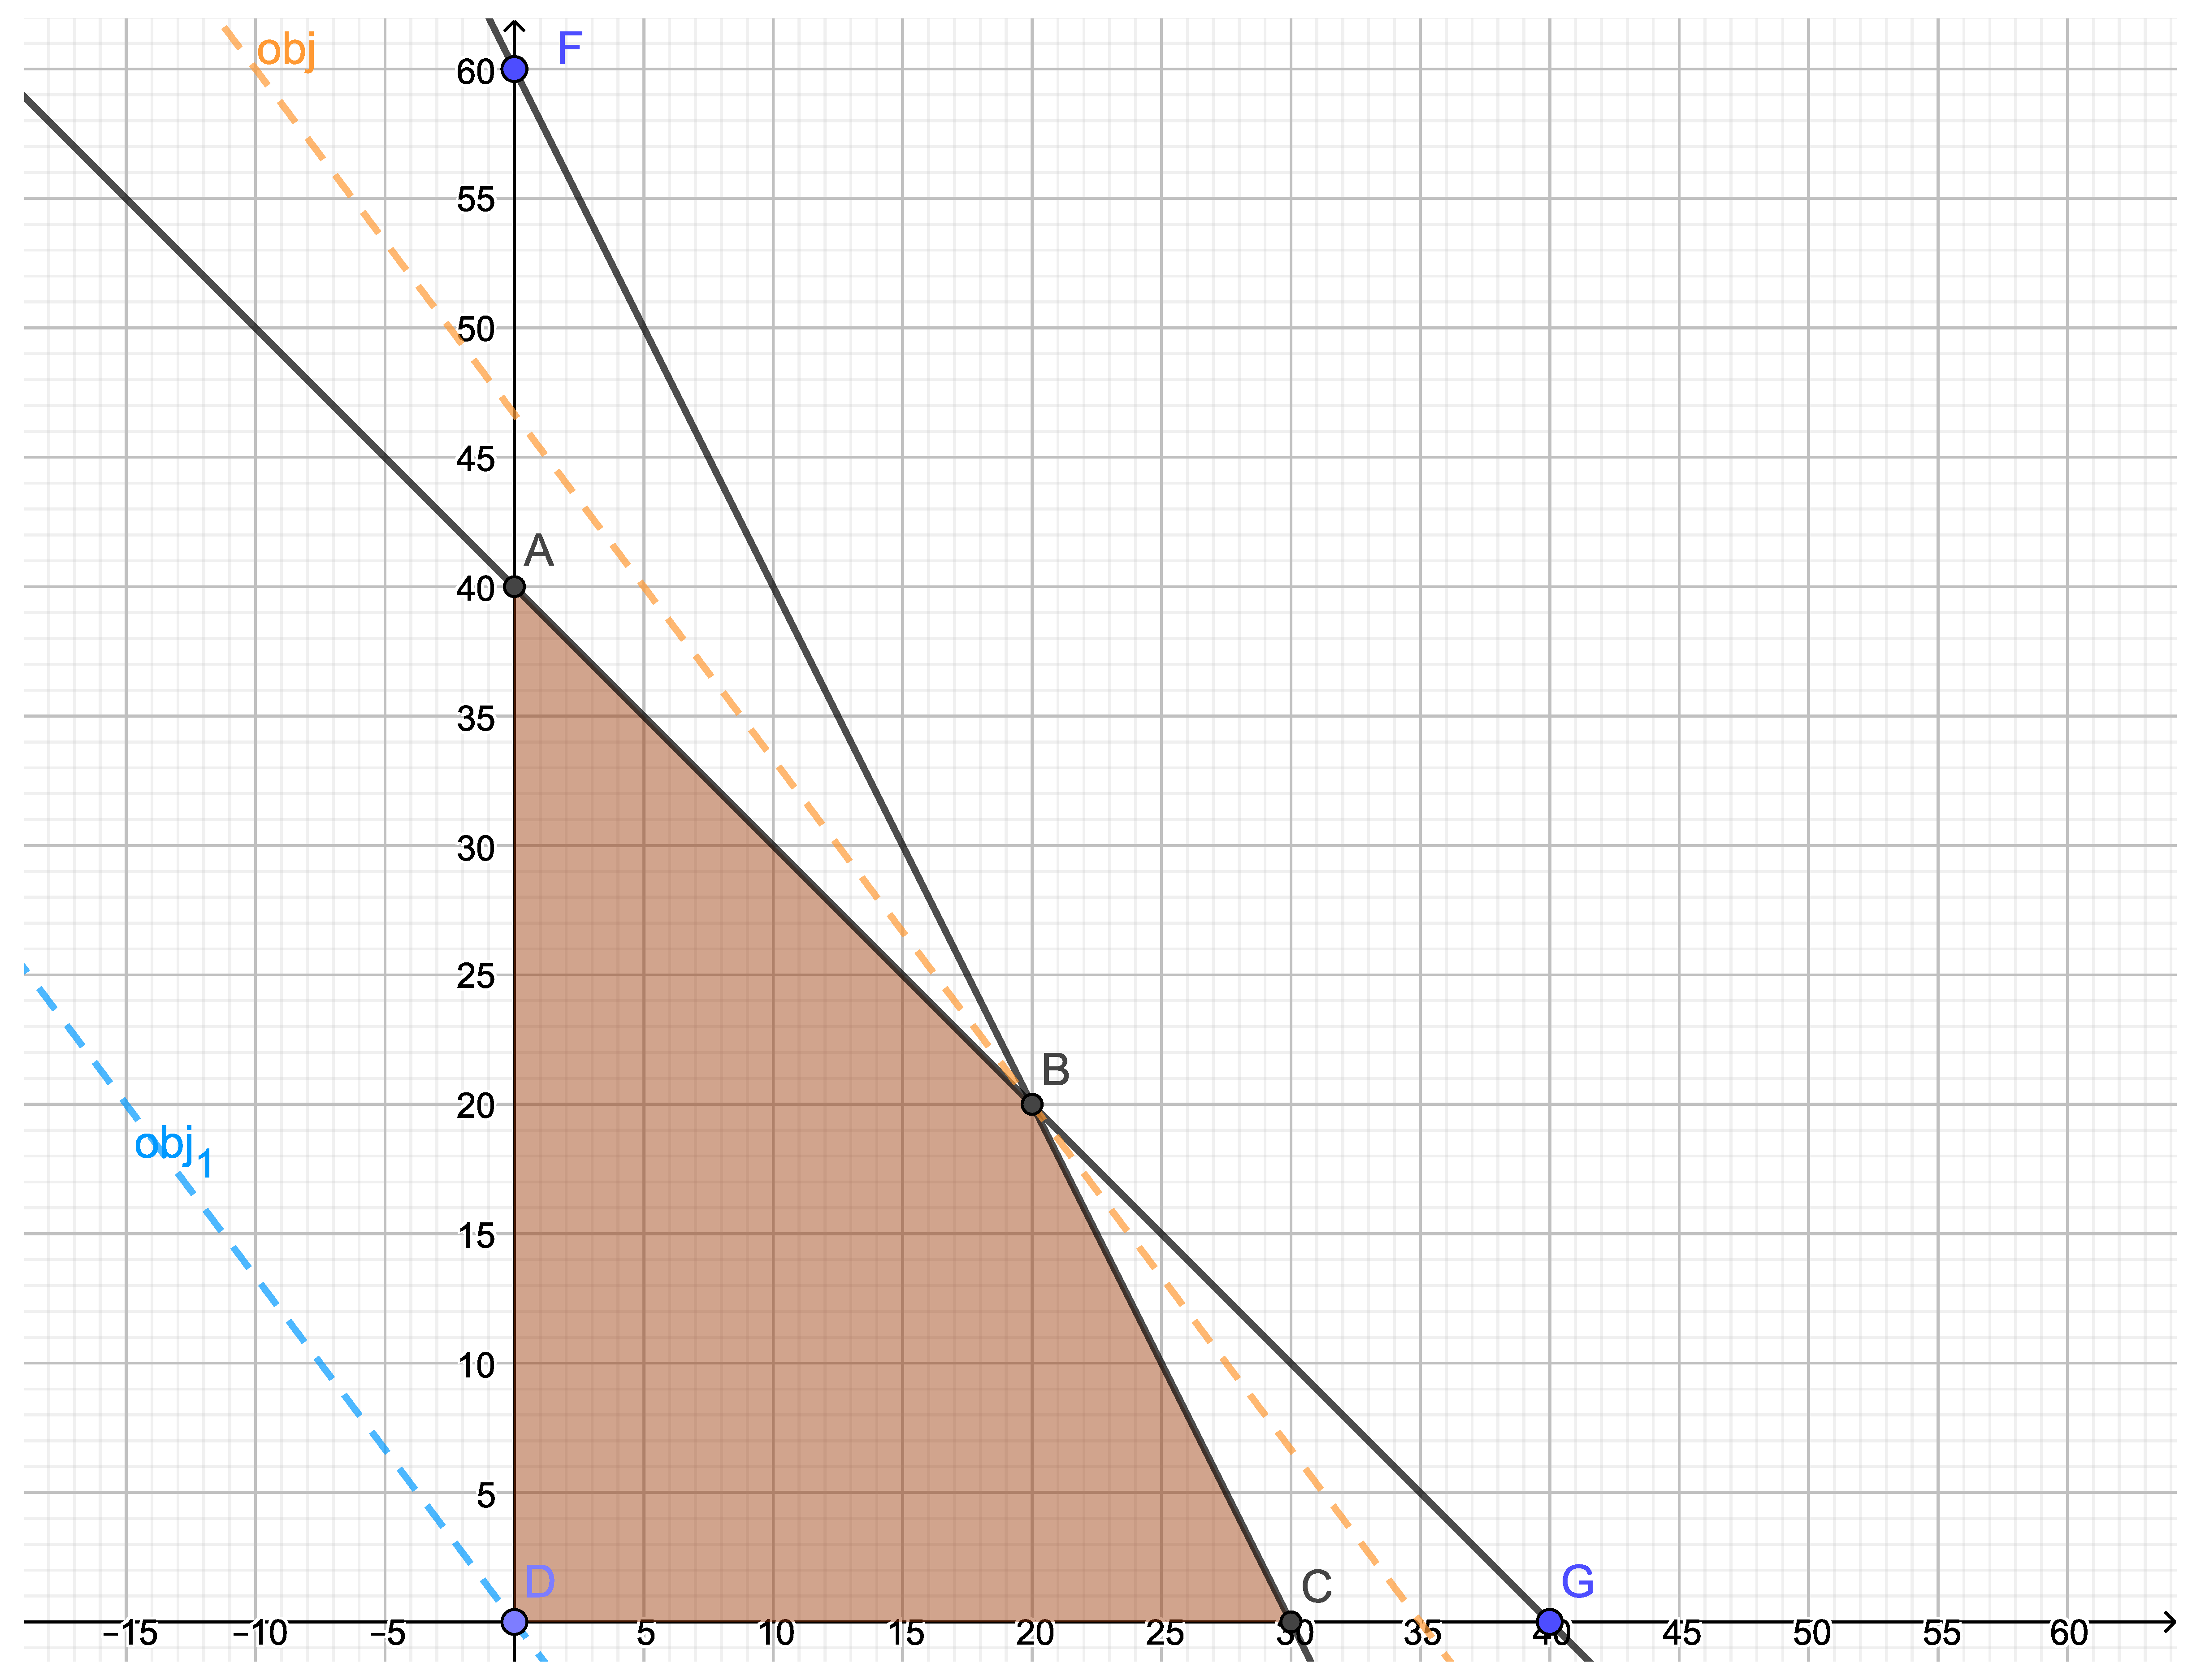
\includegraphics[width=\textwidth]{p7_primal.pdf}
        \caption{Primal (\ref{p7_primal})}
        \label{fig_primal}
    \end{subfigure}
    ~ %add desired spacing between images, e. g. ~, \quad, \qquad, \hfill etc. 
      %(or a blank line to force the subfigure onto a new line)
    \begin{subfigure}[b]{0.5\textwidth}
        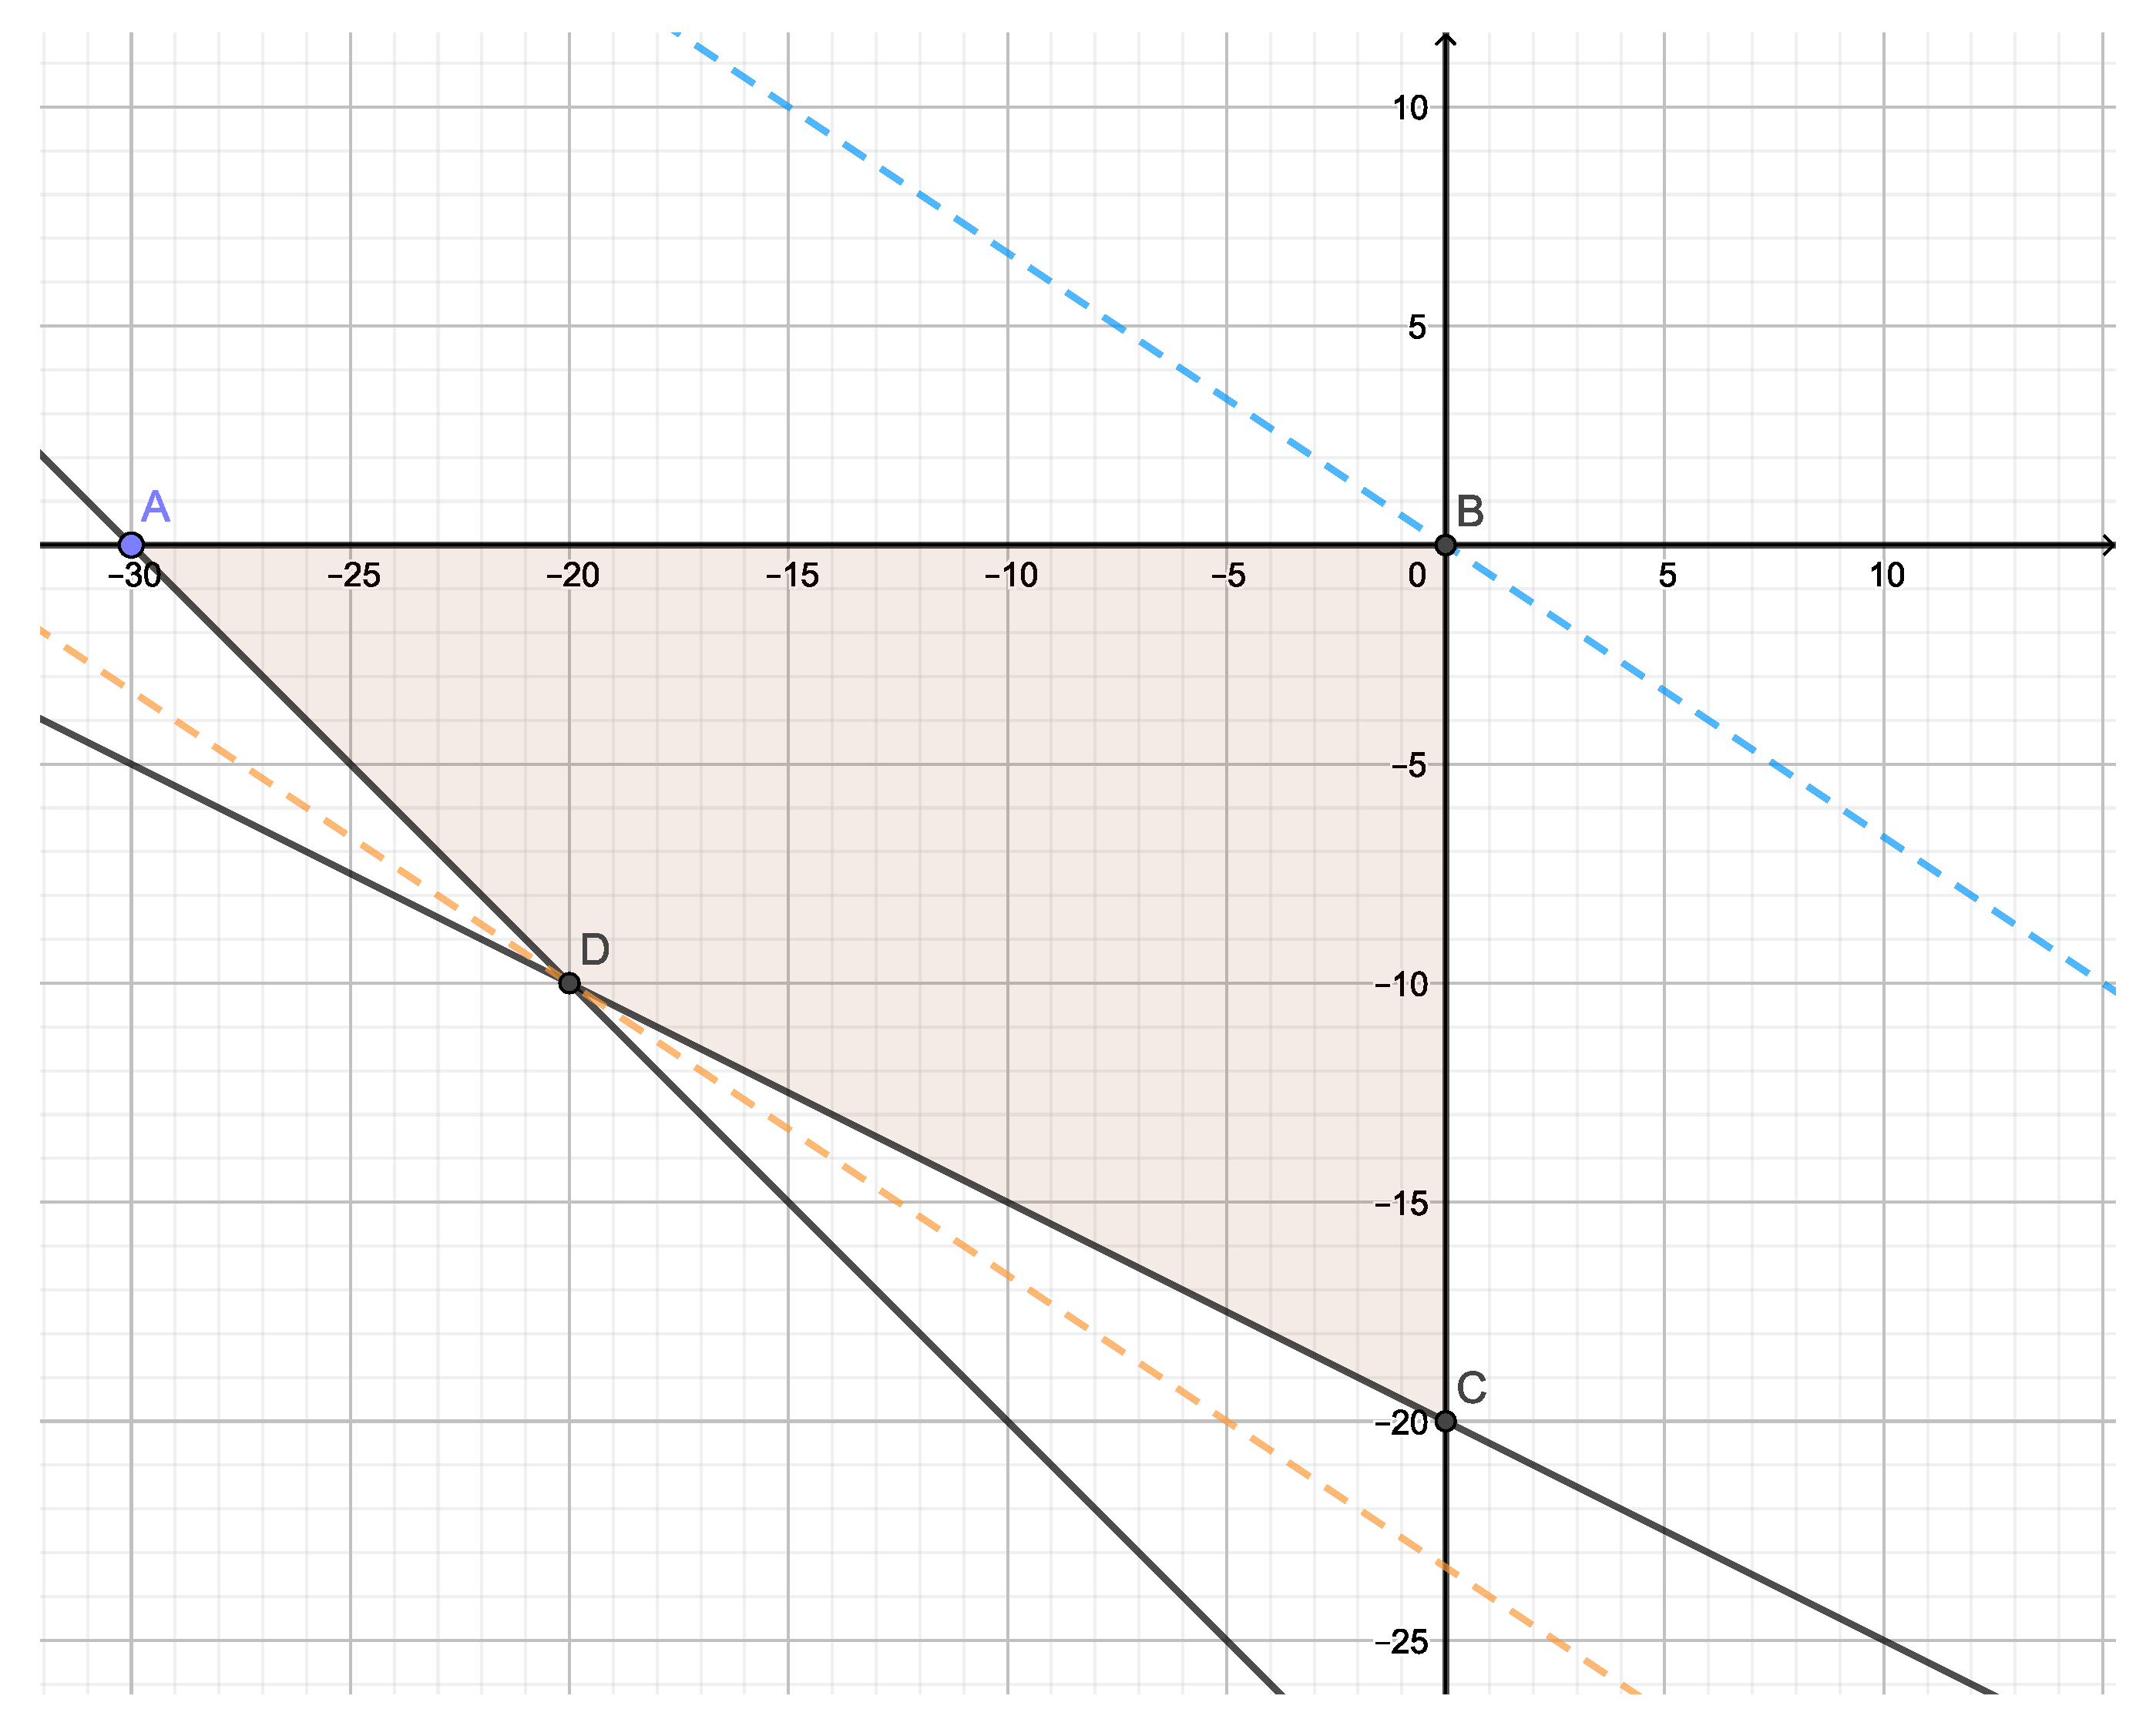
\includegraphics[width=\textwidth]{p7_dual.pdf}
        \caption{Dual (\ref{p7_dual})}
        \label{fig_dual}
    \end{subfigure}

\end{figure}

\FloatBarrier

Basic solutions of (\ref{p7_primal_std}):

$$
A = \begin{bmatrix}
1 & 1 & 1 & 0 \\
2 & 1 & 0 & 1
\end{bmatrix},  \qquad b = \begin{bmatrix}
40 \\ 60
\end{bmatrix}
$$

\FloatBarrier

\begin{table}[htbp]
\centering
\caption{Figure \ref{fig_primal}}
\label{BStable_primal}
\begin{tabular}{||c|c|c||}
\hline
 Point & Basis        & BS of (\ref{p7_primal_std}) $[x_1, x_2, x_3, x_4]^T$    \\
 \hline
A & ${[}A_2, A_4{]}$ & $[0, 40, 0, 20]^T$     \\
 \hline
B  &  $[A_1, A_2]$   & $ [20, 20, 0, 0]^T $  \ *  \\
 \hline
C  &  $[A_1, A_3]$   & $ [30, 0, 10, 0]^T $   \\
 \hline
D  &  $[A_3, A_4]$   & $ [0, 0, 40, 60]^T $    \\
\hline
F & $[A_2, A_3]$   & $ [0, 60, -20, 0]^T $    \\
\hline 
G & $[A_1, A_4]$   & $ [40, 0, 0, -20]^T $    \\
\hline 
\end{tabular}
\end{table}

\FloatBarrier

Basic solutions of (\ref{p7_primal_std}):

$$
A = \begin{bmatrix}
-1 & -2 & 1 & 0 \\
-1 & -1 & 0 & 1
\end{bmatrix},  \qquad b = \begin{bmatrix}
-40 \\ -30
\end{bmatrix}
$$

\FloatBarrier

\begin{table}[htbp]
\centering
\caption{Figure \ref{fig_dual}}
\label{BStable_dual}
\begin{tabular}{||c|c|c|c||}
\hline
 Point & Basis        & BS of (\ref{p7_dual_std}) $[z_1, z_2, z_3, z_4]^T$  & Related to Primal   \\
 \hline
A & ${[}A_1, A_3{]}$ & $[30, 0, -10, 0]^T$     &  C \\
 \hline
B  &  $[A_3, A_4]$   & $ [0, 0, -40, -30]^T $  &  D \\
 \hline
C  &  $[A_2, A_4]$   & $ [0, 20, 0, -10]^T $   &   A \\
 \hline
D  &  $[A_1, A_2]$   & $ [20, 10, 0, 0]^T $  \ $\Delta$  & B  \\
\hline 
F  &  $[A_1, A_4]$   & $ [40, 0, 0, 10]^T $  \ $\Delta$  &  G \\
\hline
G  &  $[A_2, A_3]$   & $ [0, 30, 20, 0]^T $  \ $\Delta$  & F \\
\hline
\end{tabular}
\end{table}
\FloatBarrier


Primal BFS has star "*". It is point B on Fig \ref{fig_primal}.

Dual feasible has "$\Delta$". It is point D on Fig \ref{fig_dual}.

\end{document}